\subsection{Caso d'uso UC10: Compilazione questionari generati dinamicamente}
\begin{center}
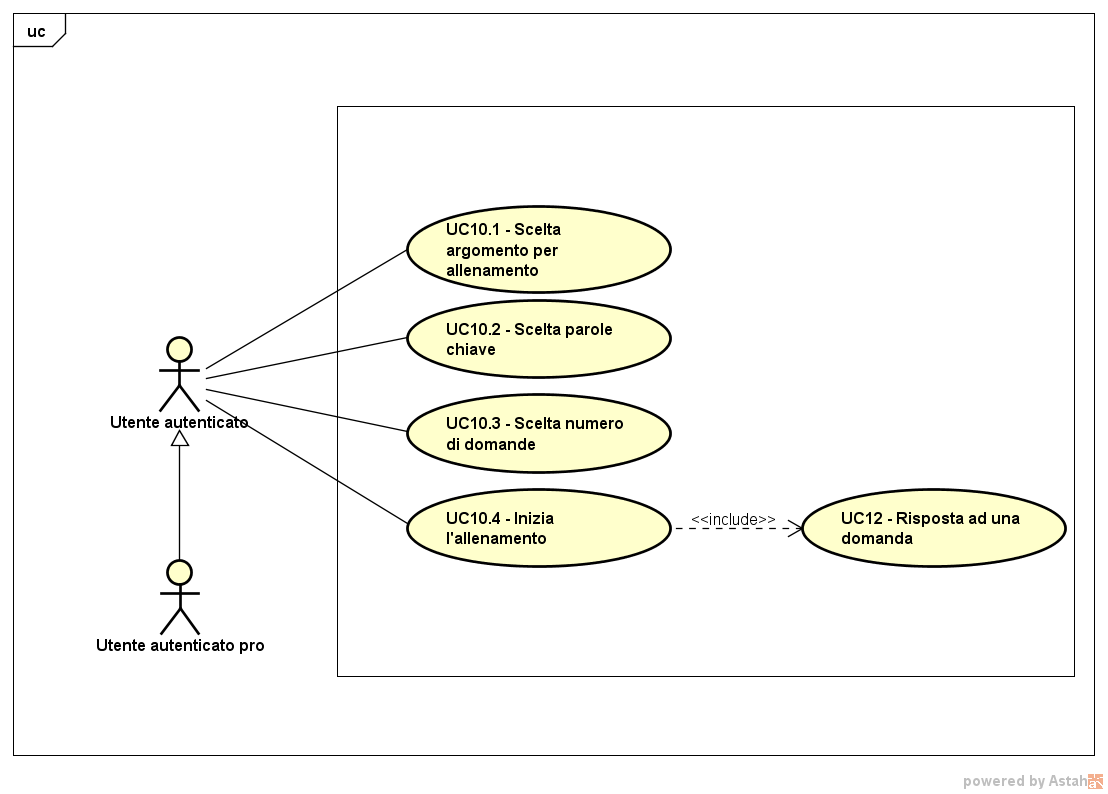
\includegraphics[scale=0.5]{UML/UC10.png}
\end{center}
\begin{itemize}
\item\textbf{Attori}: Utente autenticato, Utente autenticato pro;
\item\textbf{Descrizione}: l'utente autenticato/autenticato pro può svolgere qualsiasi tipo di questionario generato dinamicamente e infine visualizzare il risultato e il riepigolo delle risposte date;
\item\textbf{Precondizione}: l'utente autenticato/autenticato pro ha selezionato l'opzione di creazione dinamica di un questionario;
\item\textbf{Postcondizione}: l'utente ha finito di svolgere il questionario creato dinamicamente e può quindi visualizzare la valutazione finale che ha ottenuto e il riepilogo delle risposte date;
\item\textbf{Scenario principale}:
	\begin{itemize}
		\item l' utente autenticato/autenticato pro compila il questionario creato dinamicamente (UC10.1);
		\item l'utente autenticato/autenticato pro visualizza il risultato del questionario svolto (UC10.2);
	\end{itemize}
\end{itemize}

\subsubsection{Caso d'uso UC10.1: Compilazione questionario dinamico}
\begin{itemize}
	\item \textbf{Attori}: Utente autenticato/autenticato pro;
	\item \textbf{Descrizione}: l'utente autenticato/autenticato pro risponde alle domande presenti nel questionario;
	\item \textbf{Precondizione}: l'utente autenticato/autenticato pro ha selezionato un questionario dinamico e visualizza la domanda e le possibili risposte;
	\item \textbf{Postcondizione}: l'utente autenticato/autenticato pro ha coompilato il questionario dinamico.
\end{itemize}
\subsubsection{Caso d'uso UC10.2: Visualizzare il risultato del questionario dimamico svolto}
\begin{itemize}
	\item \textbf{Attori}: Utente autenticato/autenticato pro;
	\item \textbf{Descrizione}: l'utente autenticato/autenticato pro visualizza il risultato del questionario dinamico compilato;
	\item \textbf{Precondizione}: l'utente autenticato/autenticato pro ha finito di compilare il questionario dinamico;
	\item \textbf{Postcondizione}: l'utente autenticato/autenticato pro visualizza il risultato del questionario dinamico svolto 
\end{itemize}

